\section*{Part 2: Separation with SVD}

\begin{taskbox}[Part 2: introduction in the lab manual]
One of the standard and powerful techniques for data filtering based on second-order statistics is SVD, in which the data are projected onto orthogonal axes corresponding to the highest variance of the information. These variances are learned from the data (data-driven learning) and cannot be tuned in advance. In this part we want to analyze the variance content of the components using SVD.
\end{taskbox}

\question{2-1}{Reading $\mathbf{X}$, plotting the three channels and the SVD}

\begin{taskbox}
Read the data \texttt{dat.X} and display it with the provided command \texttt{ch3plot}. Then perform the SVD decomposition on \texttt{dat.X} and obtain the matrices $\mathbf{U}$, $\mathbf{S}$ and $\mathbf{V}$.
\end{taskbox}

Figure~\ref{fig:obs} shows the three observation channels in the time domain. The sample at each instant forms one point in the three-channel space; the scatter, together with the directions, is shown in the next question. Most points are concentrated around the origin, and the more distant points are associated with larger-amplitude events, including QRS complexes.

\begin{figure}[H]
\centering
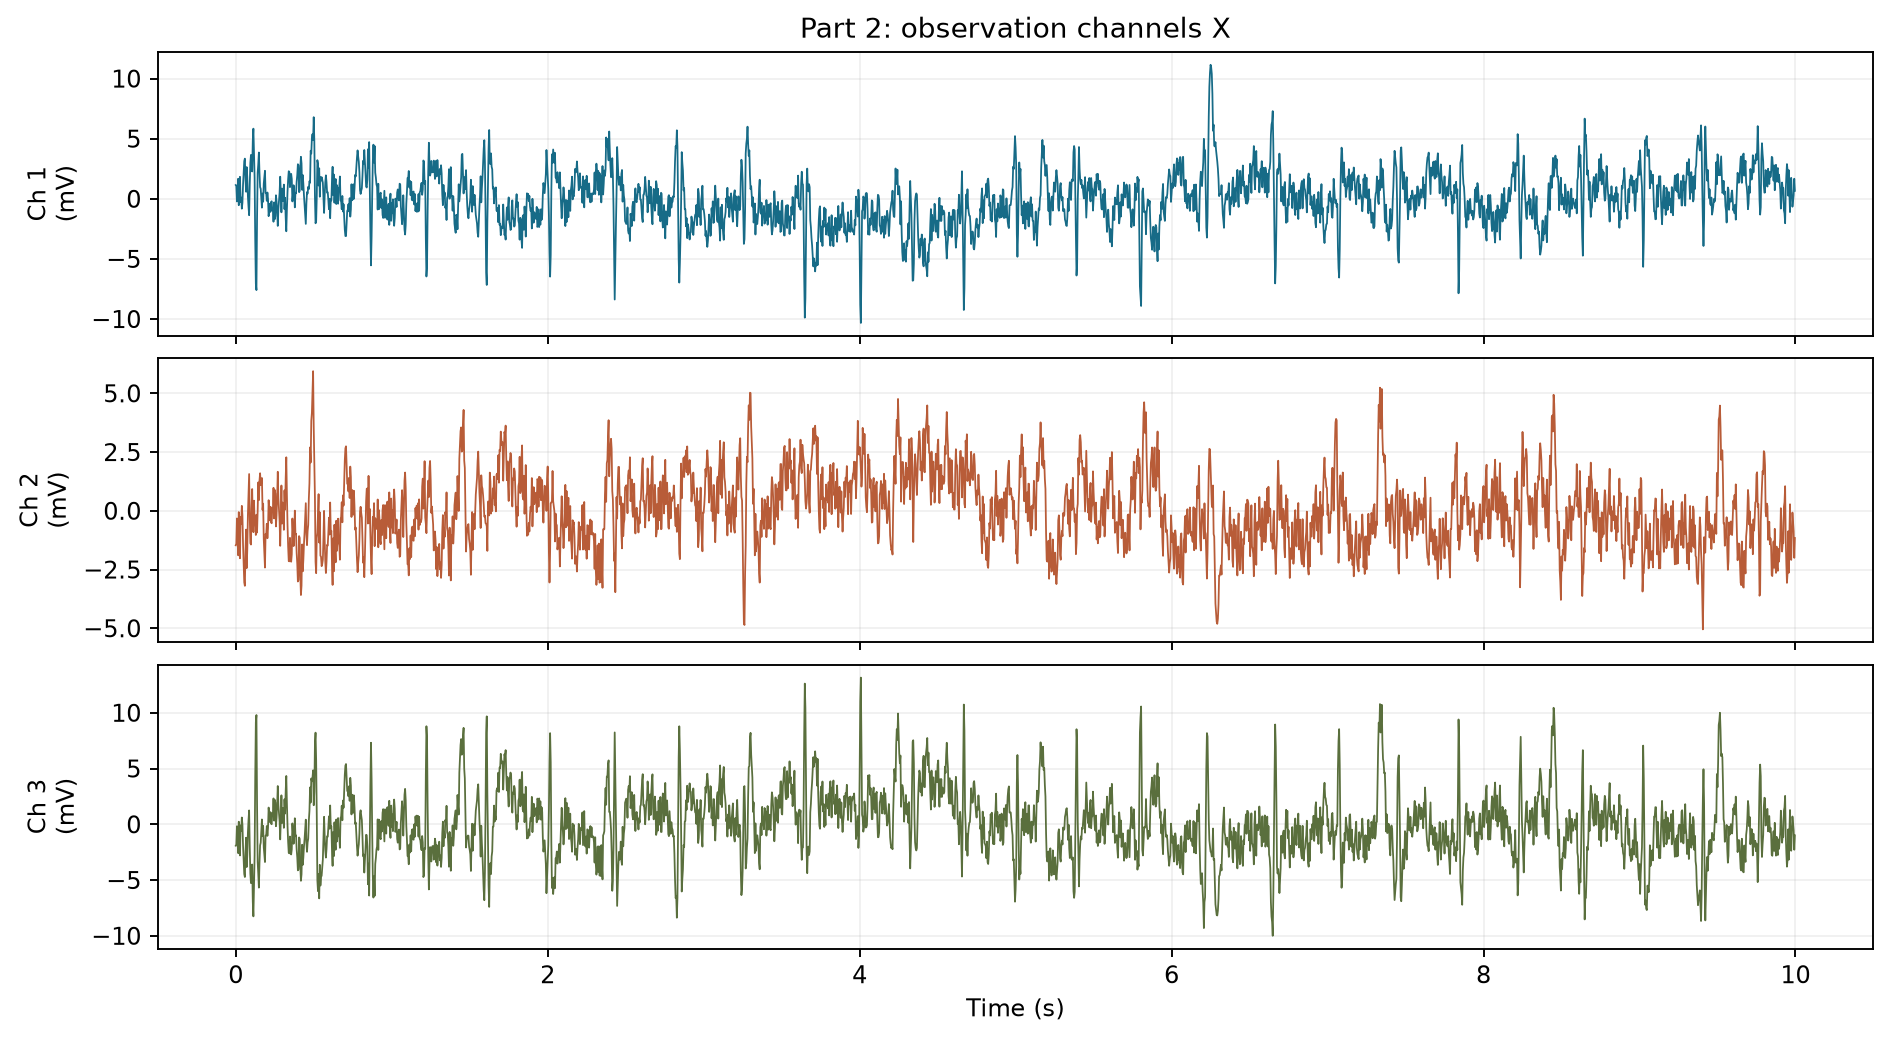
\includegraphics[width=0.95\textwidth]{fig04_observation_channels.png}
\caption{The three channels of the mixed observation from the file \texttt{X}; the full 10-second span.}
\label{fig:obs}
\end{figure}

The economy-size decomposition was computed with \texttt{numpy.linalg.svd}:
\begin{equation}
\mathbf{X}_c = \mathbf{U}\bm{\Sigma}\mathbf{V}^{T},\qquad
\mathbf{U}\in\mathbb{R}^{2560\times 3},\;
\bm{\Sigma}\in\mathbb{R}^{3\times 3},\;
\mathbf{V}\in\mathbb{R}^{3\times 3}.
\label{eq:svd}
\end{equation}
The economy version retains the same non-zero information as the full version, and building a $2560\times2560$ matrix for $\mathbf{U}$ is unnecessary. All three matrices are stored in the NPZ file. The singular values, in descending order, are 182.928983, 75.296161 and 55.465016.

\question{2-2}{Plotting the columns of $\mathbf{V}$ in three-dimensional space}

\begin{taskbox}
Plot the columns of the matrix $\mathbf{V}$ using the provided command \texttt{dv3plot}. Save the output figure in \texttt{.fig} format, together with the output matrices of the SVD method.
\end{taskbox}

\begin{figure}[H]
\centering
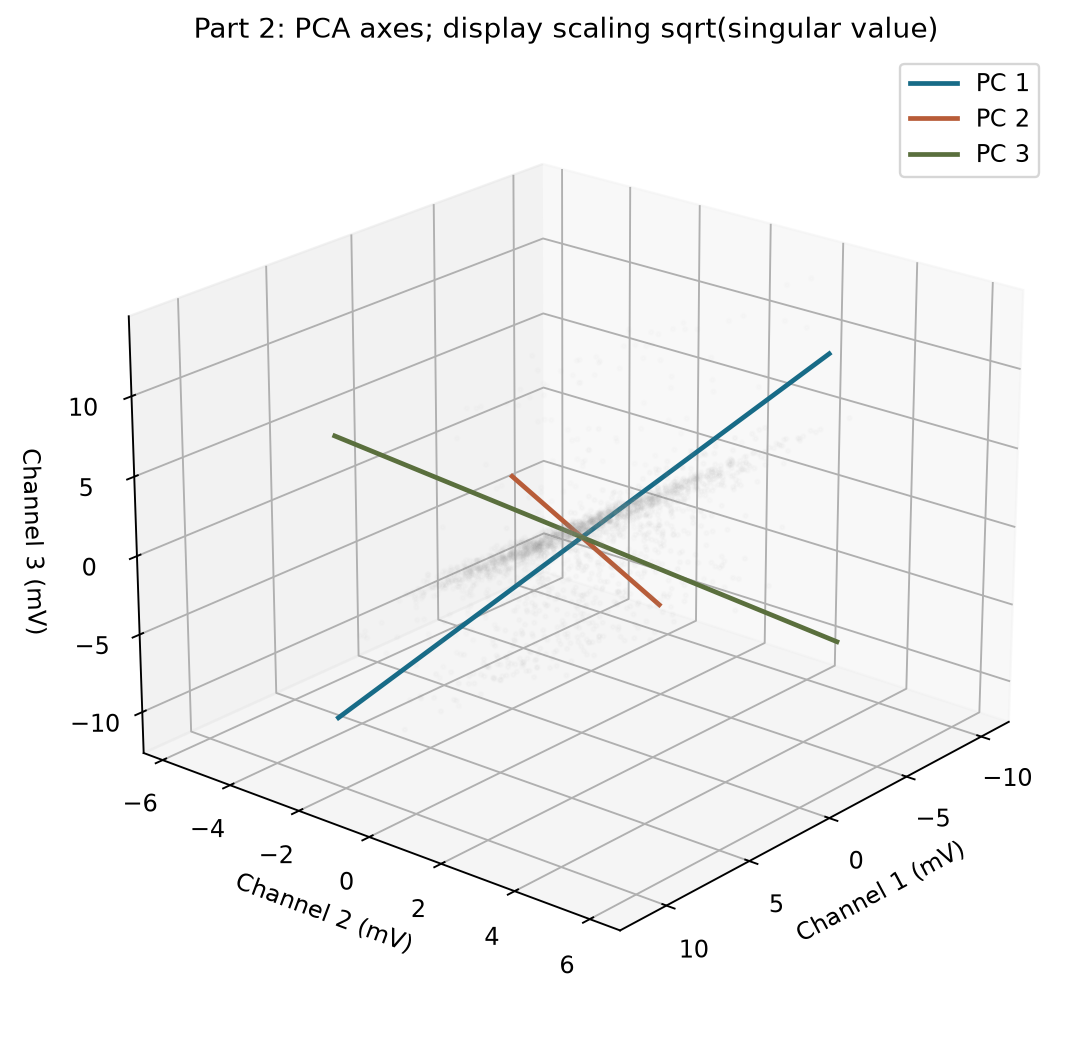
\includegraphics[width=0.72\textwidth]{fig05_pca_axes_3d.png}
\caption{Scatter of the three centered channels and the three PCA directions.}
\label{fig:pca3d}
\end{figure}

The colored lines show the directions of the columns of $\mathbf{V}$. Since $\mathbf{V}^{T}\mathbf{V}=\mathbf{I}$, these directions are orthogonal and each column has unit norm. For display, the length of each line was scaled by $\sqrt{\sigma_i}$; this display scaling is neither the eigenvalue nor the original norm of the vector. The figure is saved in PNG and SVG, and the matrices $\mathbf{U}$, $\bm{\Sigma}$ and $\mathbf{V}$ in NPZ.
\begin{equation}
\mathbf{V}\simeq
\begin{bmatrix}
-0.526476 & -0.756393 &  0.388191\\
 0.268742 & -0.581240 & -0.768074\\
 0.806598 & -0.300050 &  0.509283
\end{bmatrix}
\label{eq:V}
\end{equation}
The first direction explains the largest share of the variance; this property alone does not mean that it is a pure maternal or fetal source. As seen in the next question, several sources can contribute to a single PCA axis at the same time.

\question{2-3}{Interpreting the three columns of $\mathbf{U}$ and plotting the eigenspectrum}

\begin{taskbox}
Plot the first three columns of the matrix $\mathbf{U}$. For each of these projections, identify the dominant features (maternal, fetal, noise or mixture). Which of them is the most helpful for detecting the fetus? Also plot the eigenspectrum with the \texttt{stem} command and include it in your report.
\end{taskbox}

\begin{figure}[H]
\centering
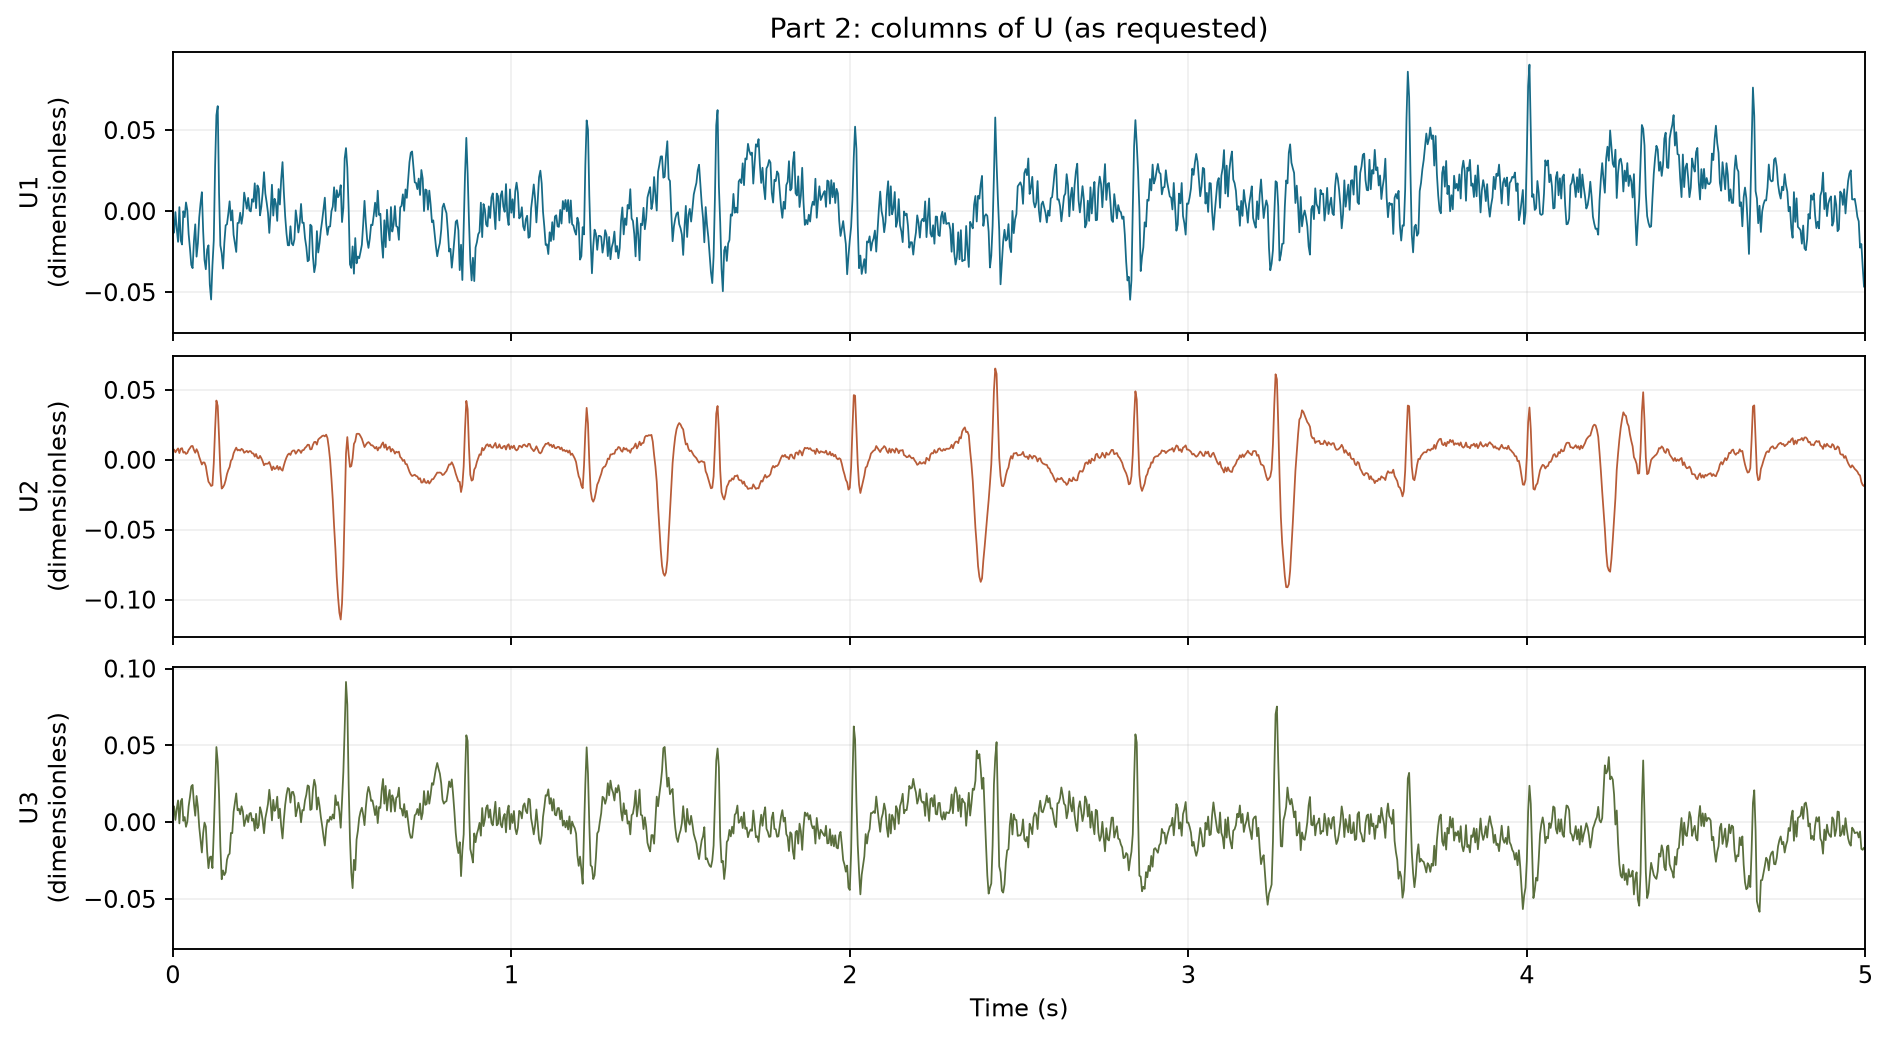
\includegraphics[width=0.95\textwidth]{fig06_svd_U_columns.png}
\caption{The first three columns of $\mathbf{U}$, as requested by the exercise; the amplitudes are normalized and dimensionless.}
\label{fig:U}
\end{figure}

\answer \textbf{Dominant features.} The first column is mixed and contains many interfering oscillations. The second column highlights the slower beats attributed to the mother, but it is not pure. The third column reveals the faster repetitions of the fetus more clearly and was chosen for the reconstruction. All columns retain some degree of mixing. In the evaluation after the separation, the absolute correlations of the first to third columns with the fetal reference are 0.546711, 0.495533 and 0.674948, respectively; this evaluation confirms the choice of the third component for this dataset.

The variance-scaled scores are $\mathbf{T}=\mathbf{U}\bm{\Sigma}=\mathbf{X}_c\mathbf{V}$; their plot is given in the appendix. The singular-value spectrum, as requested with \texttt{stem}, is drawn in Figure~\ref{fig:stem}. The covariance eigenvalue and the variance share are obtained from
\begin{equation}
\lambda_i = \frac{\sigma_i^{2}}{M-1},\qquad
p_i = \frac{\sigma_i^{2}}{\sum_j \sigma_j^{2}} .
\label{eq:lambda}
\end{equation}

\begin{figure}[H]
\centering
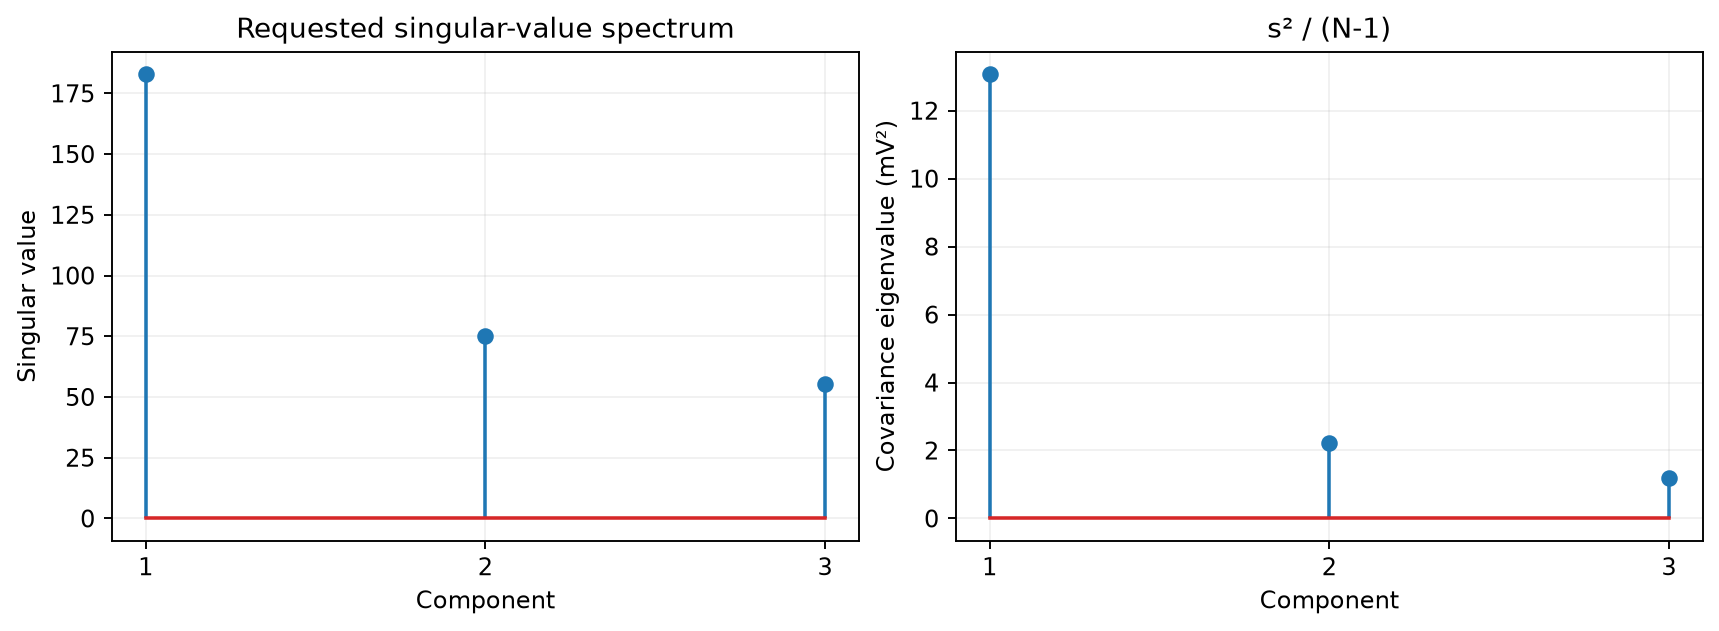
\includegraphics[width=0.92\textwidth]{fig07_singular_value_spectrum.png}
\caption{Left: spectrum of the singular values; right: spectrum of the covariance eigenvalues.}
\label{fig:stem}
\end{figure}

\begin{table}[H]
\centering
\caption{Singular values, covariance eigenvalues and variance share.}
\begin{tabular}{@{}cccc@{}}
\toprule
\textbf{Component} & $\sigma_i$ & $\lambda_i$ & \textbf{Variance share (\%)}\\
\midrule
1 & 182.928983 & 13.076597 & 79.2795\\
2 &  75.296161 &  2.215518 & 13.4320\\
3 &  55.465016 &  1.202176 &  7.2884\\
\bottomrule
\end{tabular}
\end{table}

The first component has about 79.28\% of the variance, but the third component, with a share of about 7.29\%, is more suitable for the fetus. A larger singular value is therefore not a sufficient criterion for identifying the desired signal.

\question{2-4}{Reconstructing the three fetal sensor channels with SVD and evaluating success}

\begin{taskbox}
Keep the singular value corresponding to the fetal component, set the other singular values to zero, modify the matrix $\mathbf{S}$ accordingly and put it into the SVD relation (with the same $\mathbf{U}$ and $\mathbf{V}$) to return to the fetal sensor space. Display the three recovered fetal sensor channels and describe the effect of the SVD decomposition and of the modification. Was the recovery of the fetal signal successful?
\end{taskbox}

By setting the first two singular values to zero and keeping the third, the reconstruction was carried out as
\begin{equation}
\bm{\Sigma}_f=\operatorname{diag}(0,0,\sigma_3),\qquad
\widehat{\mathbf{X}}_{f,\mathrm{SVD}}=\mathbf{U}\bm{\Sigma}_f\mathbf{V}^{T}=\sigma_3\mathbf{u}_3\mathbf{v}_3^{T}.
\label{eq:svdfetal}
\end{equation}

\begin{figure}[H]
\centering
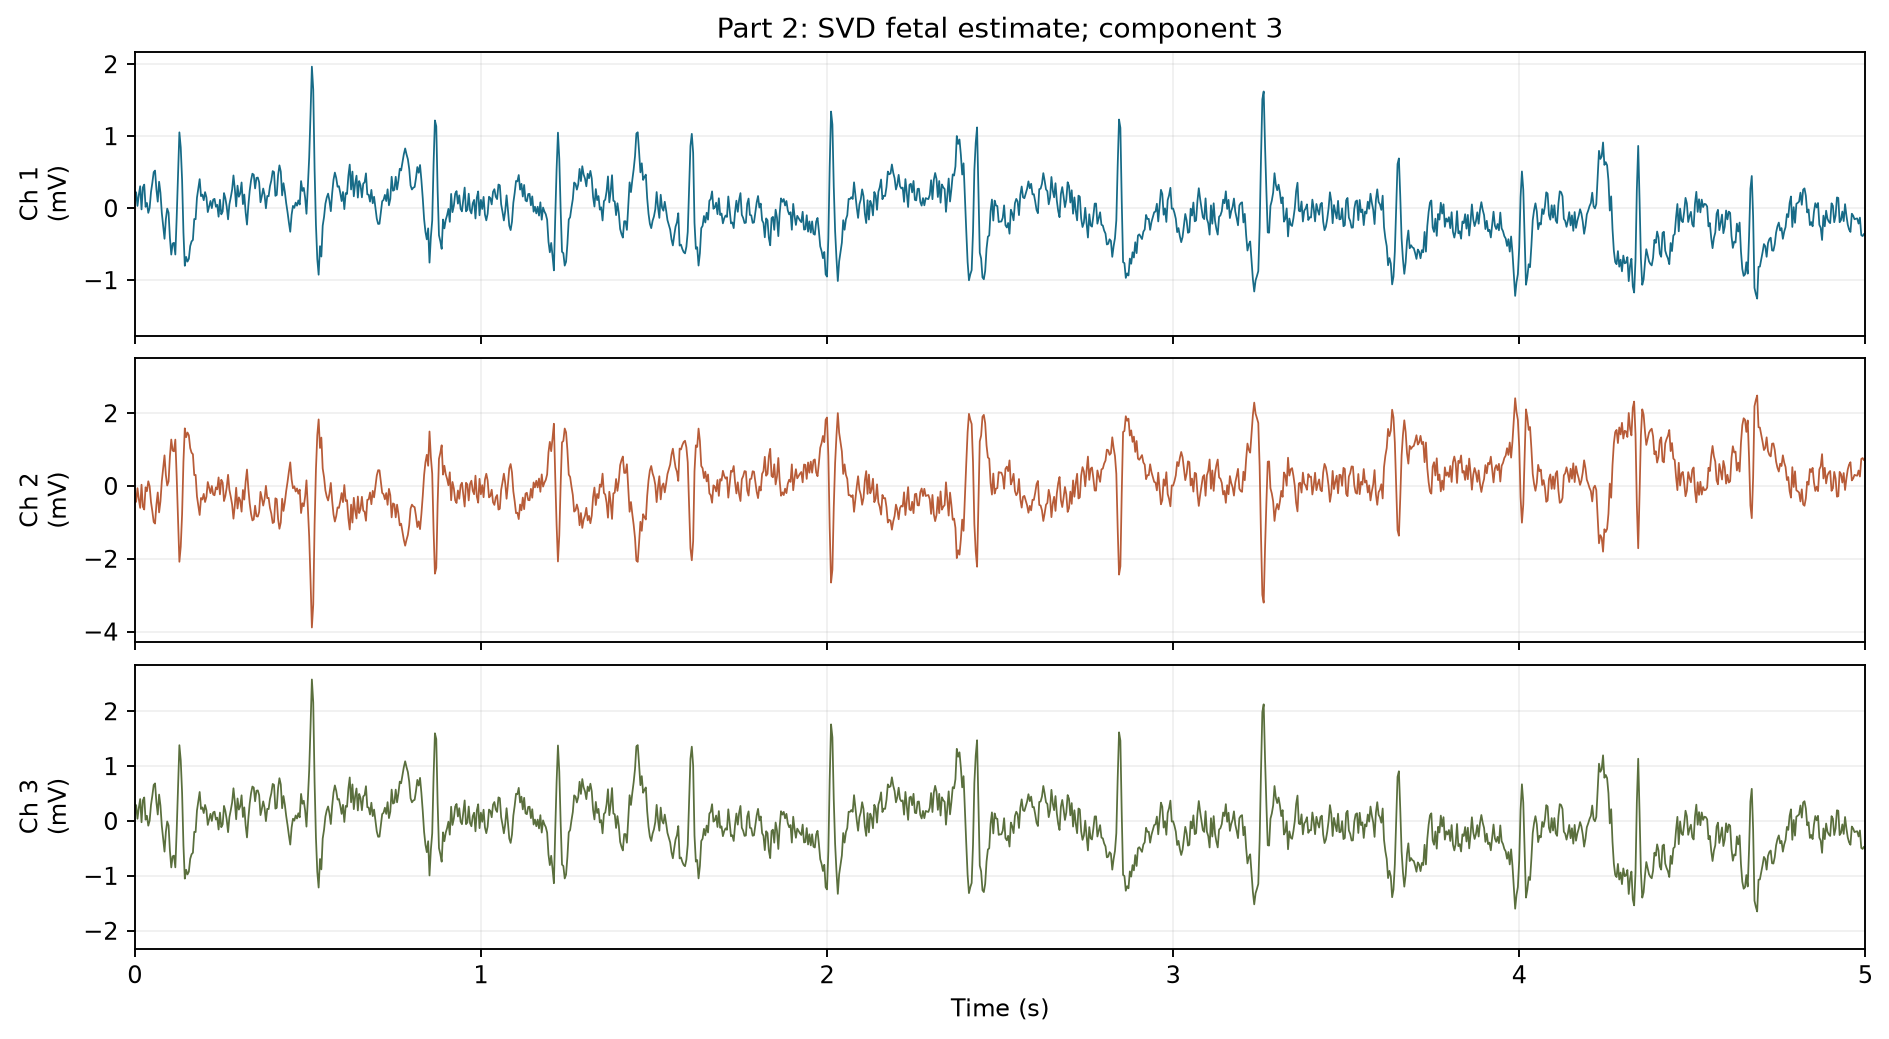
\includegraphics[width=0.95\textwidth]{fig08_svd_fetal_estimate.png}
\caption{Contribution of the third SVD component in the three sensor channels; the first five seconds are shown.}
\label{fig:svdfetal}
\end{figure}

\answer The faster beats are visible, but interfering oscillations and part of the maternal or noise contribution remain. The absolute correlation with the reference is about 0.674948, so the separation is only partial, and a complete and successful recovery of a clean waveform was not achieved. The reason is that one variance axis in SVD does not necessarily coincide with one independent source.

The three reconstructed channels share one temporal shape with different coefficients, because the reconstruction has rank one. The sign difference between the channels arises from the sensor direction of $\mathbf{v}_3$. Flipping the signs of $\mathbf{u}_3$ and $\mathbf{v}_3$ simultaneously does not change the reconstruction.
